\subsection{Study of the Relativistic NN Bound System}

One of the important issues in studying nuclear structure  at short distances is the 
relativistic description of the bound system.  This is an important issue also in 
understanding the QCD medium effect with recent studies indicating that  parton distribution 
modifications  in nuclei are proportional to the high momentum component of nuclear wave function~\cite{Weinstein:2010rt}.

The deuteron is the simplest bound system and naturally any self-consistent attempt  to understand the 
relativistic effects in the bound nuclear systems  should start with the deuteron. 
The issue of the relativistic description of the deuteron has a long history with extensive research that started in the late 1970's~\cite{Gross:1982nz,Buck:1979ff,Frankfurt:1977vc,Frankfurt:1981mk}.

Experimental studies of relativistic effects in the deuteron  up to now include the large $Q^2$ elastic 
$ed$ scattering~\cite{Alexa:1998fe}, however  
due to complexities  in the reaction mechanism~\cite{VanOrden:1995eg} the relativistic effects were 
difficult to isolate.

Inclusive D$(e,e')$X experiments from tensor-polarized deuterons at  $Q^2>1$~GeV$^2$ and in the $x>1$ region gives 
a new possibility to probe the relativistic structure of the deuteron.  In this case the use of the tensor polarized
deuteron allows us to prepare the nucleus in the most compact state in which, due to the absence of the 
pure S-wave contribution, the system in average is sensitive to the higher nucleon momenta in the deuteron.
At large $Q^2>1$ GeV$^2$ kinematics, the probed longitudinal momenta of the bound nucleon is given by $p_z \approx m_N(1-x)$, 
or the light cone momentum fraction $\alpha \ge x$. Because of these kinematic conditions and the enhancement of the 
D-wave contribution from tensor polarization, a measurable relativistic effects is expected already at $x\approx 1.2$.  Such an early onset of the relativistic effects indicates that they can be separated from the choice of NN potentials, which dominate at $x>1.4$. 

%The biggest advantage is that one expects less uncertainty at $x<1.3$ due to the choice of the NN potential and reaction dynamics due to relatively small values of the bound nucleon momenta involved ($\ge 200~\mathrm{MeV}/c$).

The sensitivity to relativistic effects is estimated using the theoretical calculations based on two 
very different approaches.   The first approach treats the  virtuality of the bound nucleon within a
description of the deuteron in the lab frame by treating the interacting nucleon as being 
virtual (virtual nucleon, or VN approximation). This is accomplished by taking the residue over the energy of the spectator nucleon.
In this case, the deuteron wave function satisfies the covariant equation of the two-nucleon bound system 
with one spectator being on energy shell~\cite{Sargsian:2009hf,Gross:2010qm}.

Another approach is based on the observation that high energy processes
evolve along the light-cone (LC).  Therefore, it is natural to describe the 
reaction within the light-cone non-covariant framework \cite{Frankfurt:1981mk}. 
Negative energy states do not enter in this case, though one has to take into 
account so called instantaneous interactions.
In the approximation when non-nucleonic degrees of freedom 
%in the deuteron wave function 
can be neglected, assuming rotational invariance of the LC deuteron wave function around its quantization axis, the relativistic wave function can be related to the nonrelativistic wave function through the introduction of LC $pn$ relative momentum~\cite{Frankfurt:1981mk, Miller:2009fc},

%one can relate the light-cone wave functions to those calculated in the lab frame by introducing the LC $pn$ relative three momentum,
\begin{equation}
k=\sqrt{{m^2+p_t^2\over \alpha(2-\alpha)} - m^2}.
\end{equation}

In Fig.~\ref{fig:misak}, the prediction for VN~\cite{Sargsian:2009hf} and LC~\cite{Frankfurt:1993sp} approximations are given 
for the highest $Q^2$ kinematics proposed. As was previously mentioned, a measurable 
difference is predicted to be observable already at $x\ge 1.2$.
% where one expects little uncertainty due to the choice of the wave function.  
 
 

\begin{figure}
\begin{center}
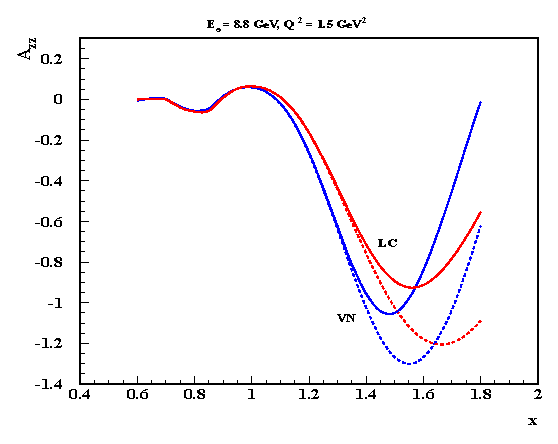
\includegraphics[width=0.49\textwidth]{figs/mark_misak_azz.eps}  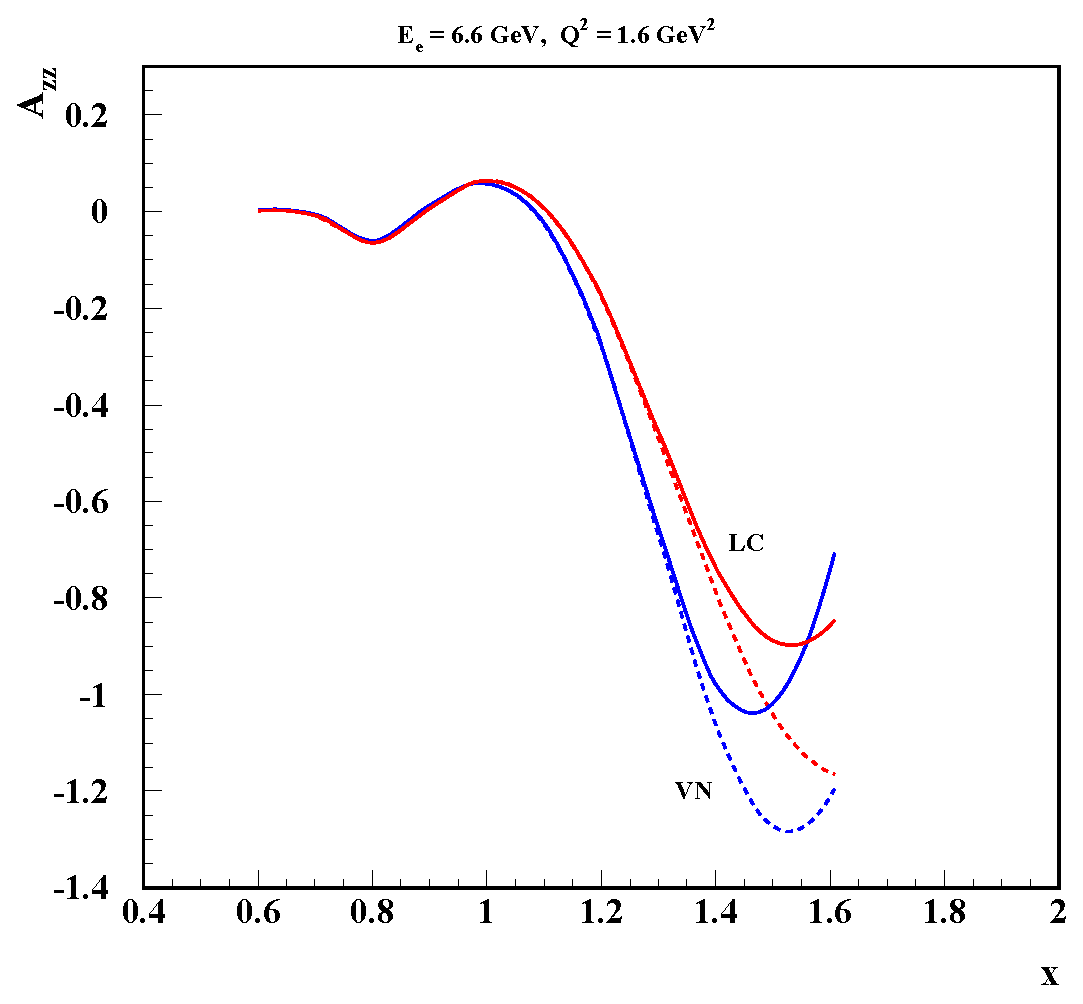
\includegraphics[width=0.49\textwidth]{figs/h2_ratio_t20_sigma.eps}
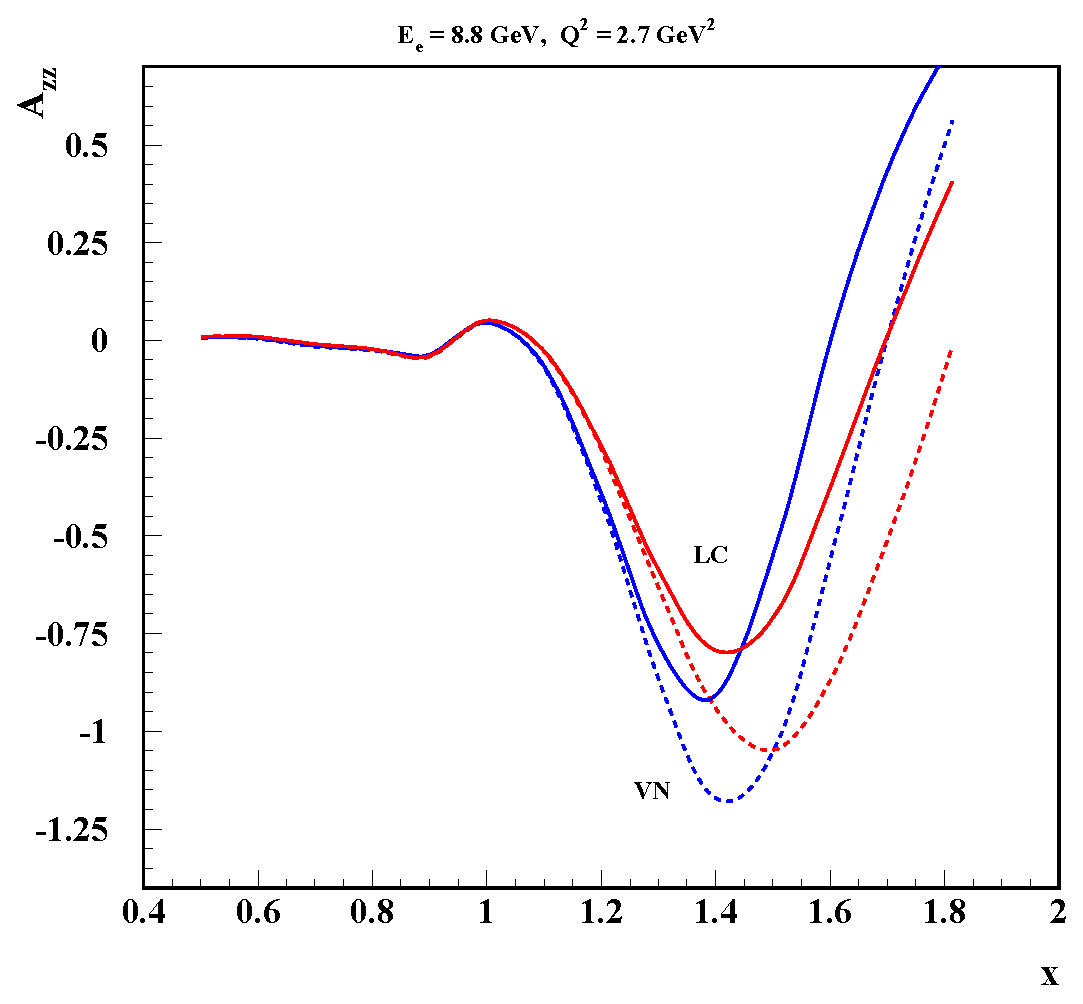
\includegraphics[width=0.49\textwidth]{figs/h1_ratio_t20_sigma.eps}
\caption{\label{fig:misak} The $A_{zz}$ observable calculated at $Q^2=1.5$, 1.8, and $2.9~(\mathrm{GeV}/c)^2$ using the light-cone (red) and virtual nucleon (blue) models with NN potential inputs of AV18 (solid) and CDBonn (dotted). Calculations provided by M. Sargsian and M. Strikman~\cite{Sargsian:2014fla,misak-convo}.}
\end{center}
\end{figure}

